\documentclass{article}
\usepackage{amsmath}
\usepackage{graphicx} % Required to insert images
\usepackage[margin=0.2in]{geometry}
\begin{document}
	
\begin{center}
	{\Large Ball Tracker Robot}
\end{center}

\begin{center}
	{\large Note: we set the configuration in such a way \\
		so that the robot sits up straight when all of $\theta_{1}, \theta_{2}, \theta_{3}, \theta_{4}$ are 0. \\ That is, we are using $\theta_{1}+90$ and $ \theta_{2}+90$.}
\end{center}

\begin{center}
	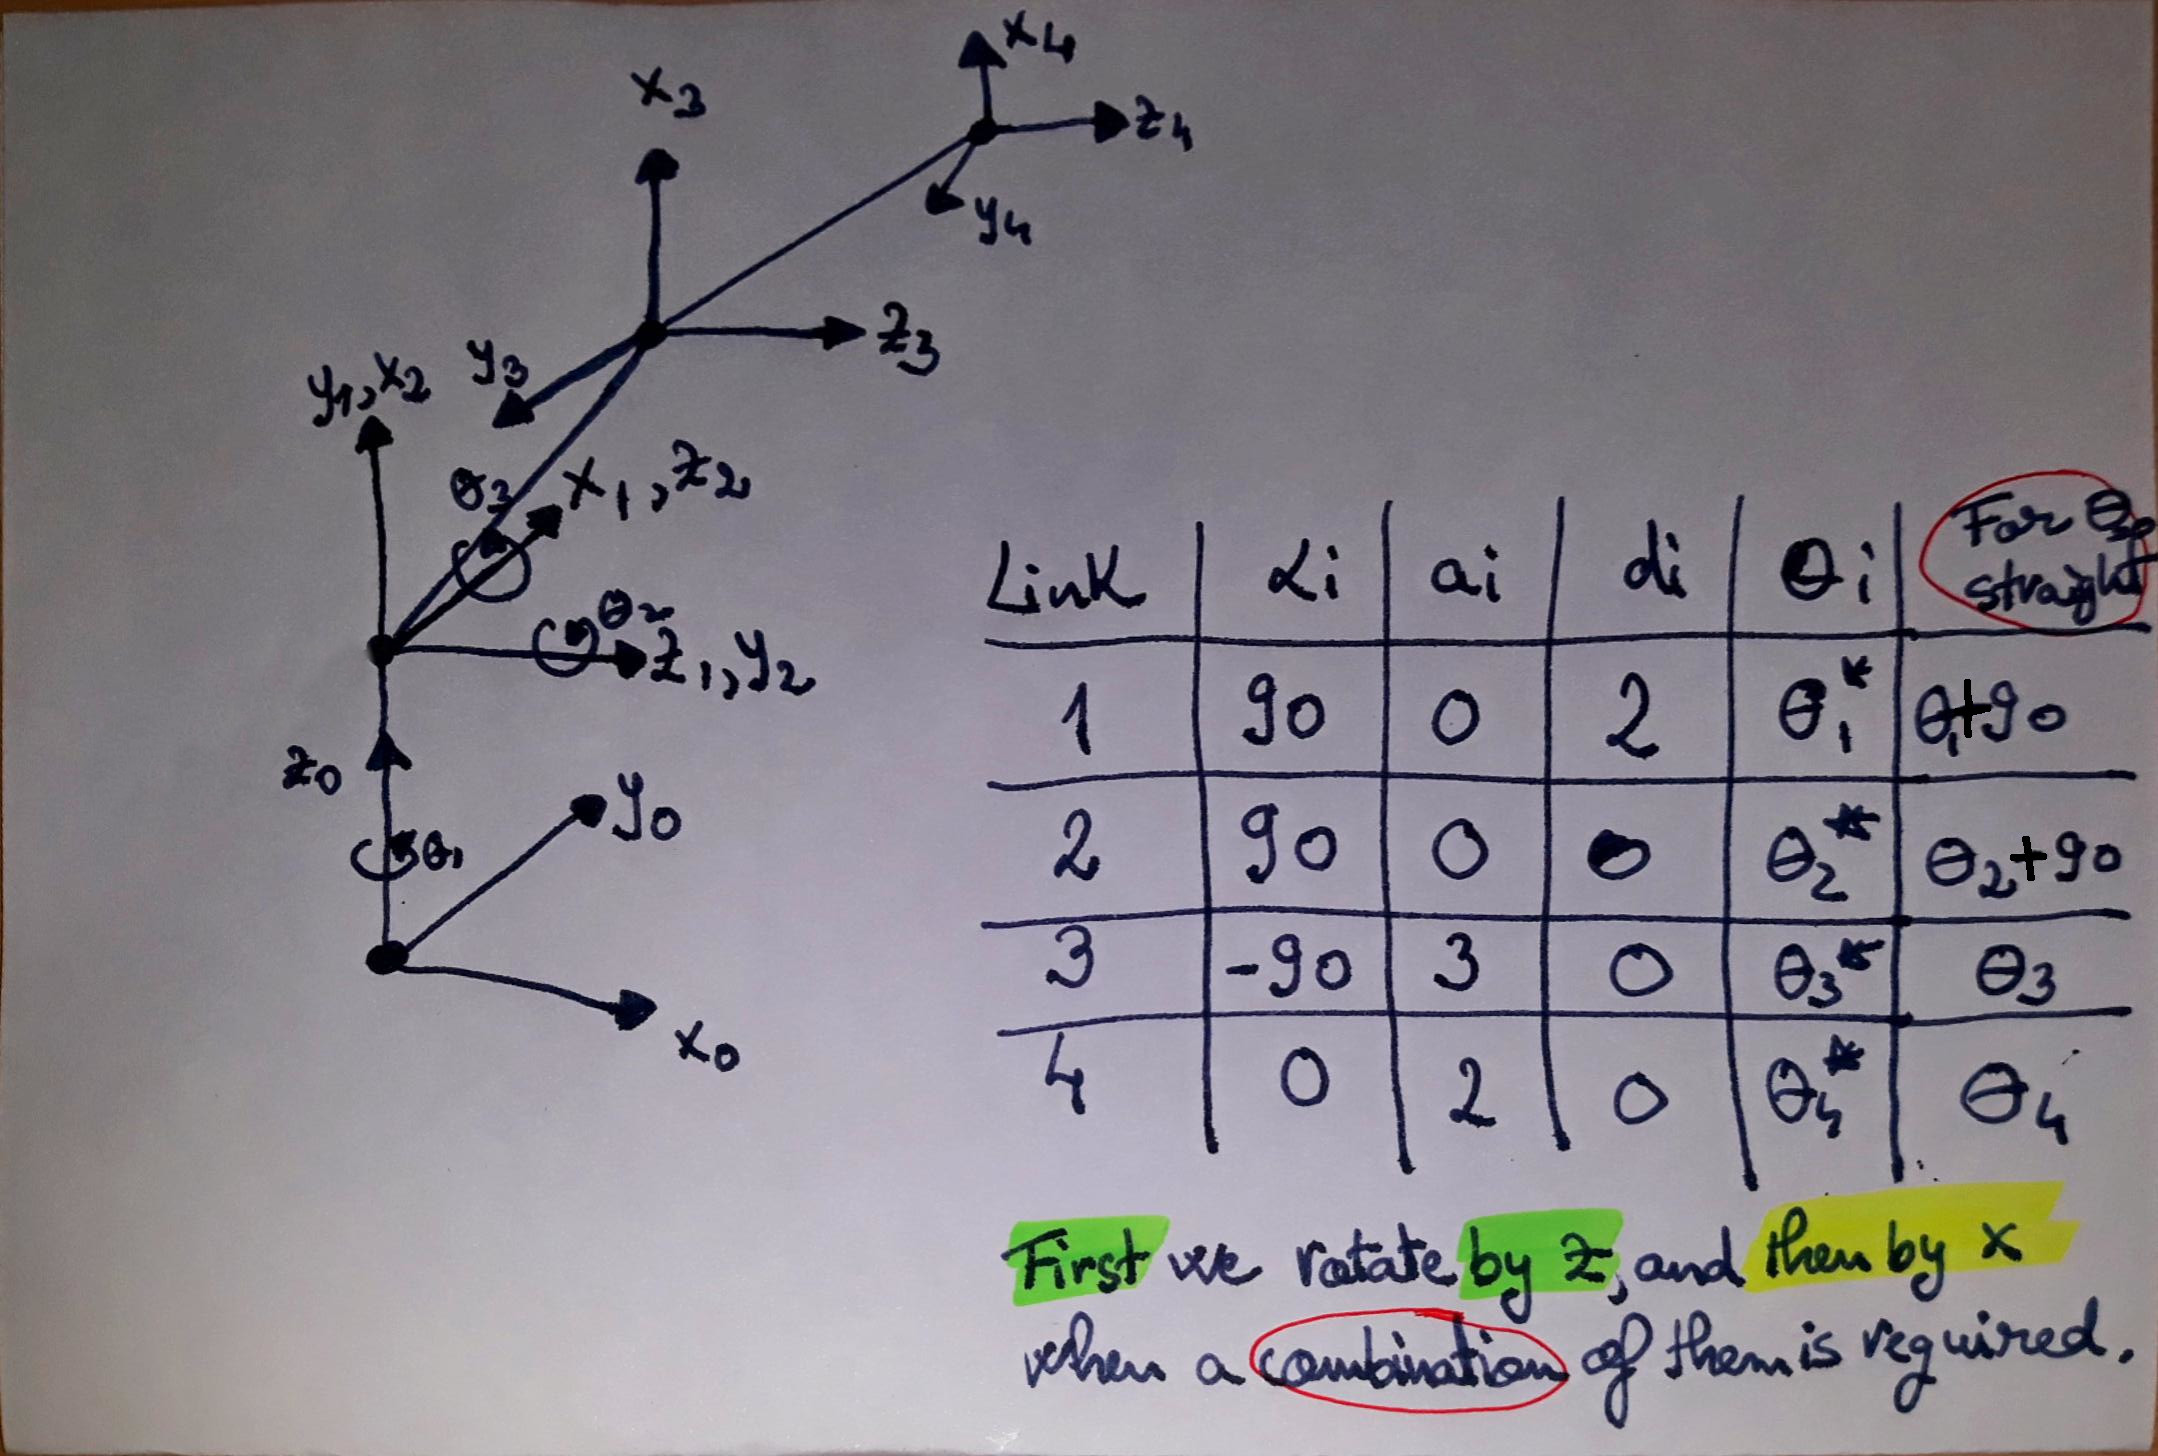
\includegraphics[width=0.9\textwidth]{Configuration}
\end{center}

\newpage

\begin{center}
	{\Large Forward Kinematics}
\end{center}
{\large
\[
Remember: \cos (a+b) = \cos (a)\cos (b) - \sin (a)\sin (b),  \sin (a+b) = \sin(a)\cos(b) + \sin(b)\cos(a)
\]
\[
\cos \theta_{x} = c_{x},  \sin \theta_{x} = s_{x}
\]
\[
A=T_{\theta}T_{d}T_{\alpha}T_{a} 
\]
\[
A1=T_{\theta_{1}+90}T_{d=2}T_{\alpha=90}
  =
  \begin{bmatrix}
    \cos (\theta_{1} + \frac{\pi}{2}) & - \sin (\theta_{1} + \frac{\pi}{2}) & 0 & 0 \\
    \sin (\theta_{1} + \frac{\pi}{2}) & \cos (\theta_{1} + \frac{\pi}{2}) & 0 & 0 \\
    0 & 0 & 1 & 0 \\
    0 & 0 & 0 & 1
  \end{bmatrix}
  \begin{bmatrix}
  1 & 0 & 0 & 0 \\
  0 & 1 & 0 & 0 \\
  0 & 0 & 1 & 2 \\
  0 & 0 & 0 & 1
  \end{bmatrix}
  \begin{bmatrix}
  1 & 0 & 0 & 0 \\
  0 & 0 & -1 & 0 \\
  0 & 1 & 0 & 0 \\
  0 & 0 & 0 & 1
  \end{bmatrix}
  =
  \begin{bmatrix}
  -s_{1} & 0 & c_{1} & 0 \\
  c_{1} & 0 & s_{1} & 0 \\
  0 & 1 & 0 & 2 \\
  0 & 0 & 0 & 1
  \end{bmatrix}
\]
\[
A2=T_{\theta_{2}+90}T_{\alpha=90}
=
\begin{bmatrix}
\cos (\theta_{2} + \frac{\pi}{2}) & - \sin (\theta_{2} + \frac{\pi}{2}) & 0 & 0 \\
\sin (\theta_{2} + \frac{\pi}{2}) & \cos (\theta_{2} + \frac{\pi}{2}) & 0 & 0 \\
0 & 0 & 1 & 0 \\
0 & 0 & 0 & 1
\end{bmatrix}
\begin{bmatrix}
1 & 0 & 0 & 0 \\
0 & 0 & -1 & 0 \\
0 & 1 & 0 & 0 \\
0 & 0 & 0 & 1
\end{bmatrix}
=
\begin{bmatrix}
-s_{2} & 0 & c_{2} & 0 \\
c_{2} & 0 & s_{2} & 0 \\
0 & 1 & 0 & 0 \\
0 & 0 & 0 & 1
\end{bmatrix}
\]
\[
A3=T_{\theta_{3}}T_{a=3}T_{\alpha=-90}
=
\begin{bmatrix}
c_{3} & - s_{3} & 0 & 0 \\
s_{3} & c_{3} & 0 & 0 \\
0 & 0 & 1 & 0 \\
0 & 0 & 0 & 1
\end{bmatrix}
\begin{bmatrix}
1 & 0 & 0 & 3 \\
0 & 1 & 0 & 0 \\
0 & 0 & 1 & 0 \\
0 & 0 & 0 & 1
\end{bmatrix}
\begin{bmatrix}
1 & 0 & 0 & 0 \\
0 & 0 & 1 & 0 \\
0 & -1 & 0 & 0 \\
0 & 0 & 0 & 1
\end{bmatrix}
=
\begin{bmatrix}
c_{3} & 0 & -s_{3} & 3c_{3} \\
s_{3} & 0 & c_{3} & 3s_{3} \\
0 & -1 & 0 & 0 \\
0 & 0 & 0 & 1
\end{bmatrix}
\]
\[
A4=T_{\theta_{4}}T_{a=2}
=
\begin{bmatrix}
c_{4} & - s_{4} & 0 & 0 \\
s_{4} & c_{4} & 0 & 0 \\
0 & 0 & 1 & 0 \\
0 & 0 & 0 & 1
\end{bmatrix}
\begin{bmatrix}
1 & 0 & 0 & 2 \\
0 & 1 & 0 & 0 \\
0 & 0 & 1 & 0 \\
0 & 0 & 0 & 1
\end{bmatrix}
=
\begin{bmatrix}
c_{4} & - s_{4} & 0 & 2c_{4} \\
s_{4} & c_{4} & 0 & 2s_{4} \\
0 & 0 & 1 & 0 \\
0 & 0 & 0 & 1
\end{bmatrix}
\]
\\
\\
\[
A1A2A3=
\begin{bmatrix}
-s_{1} & 0 & c_{1} & 0 \\
c_{1} & 0 & s_{1} & 0 \\
0 & 1 & 0 & 2 \\
0 & 0 & 0 & 1
\end{bmatrix}
\begin{bmatrix}
-s_{2} & 0 & c_{2} & 0 \\
c_{2} & 0 & s_{2} & 0 \\
0 & 1 & 0 & 0 \\
0 & 0 & 0 & 1
\end{bmatrix}
\begin{bmatrix}
c_{3} & 0 & -s_{3} & 3c_{3} \\
s_{3} & 0 & c_{3} & 3s_{3} \\
0 & -1 & 0 & 0 \\
0 & 0 & 0 & 1
\end{bmatrix}
\]
\[
=
\begin{bmatrix}
s_{1}s_{2} & c_{1} & -s_{1}c_{2} & 0 \\
-c_{1}s_{2} & s_{1} & c_{1}c_{2} & 0 \\
c_{2} & 0 & s_{2} & 2 \\
0 & 0 & 0 & 1
\end{bmatrix}
\begin{bmatrix}
c_{3} & 0 & -s_{3} & 3c_{3} \\
s_{3} & 0 & c_{3} & 3s_{3} \\
0 & -1 & 0 & 0 \\
0 & 0 & 0 & 1
\end{bmatrix}
\]
\[
=
\begin{bmatrix}
s_{1}s_{2}c_{3} + c_{1}s_{3} & s_{1}c_{2} & -s_{1}s_{2}s_{3} + c_{1}c_{3} & 3s_{1}s_{2}c_{3} + 3c_{1}s_{3} \\
-c_{1}s_{2}c_{3} + s_{1}s_{3} & -c_{1}c_{2} & c_{1}s_{2}s_{3} + s_{1}c_{3} & -3c_{1}s_{2}c_{3} + 3s_{1}s_{3} \\
c_{2}c_{3} & -s_{2} & -c_{2}s_{3} & 3c_{2}c_{3}+2 \\
0 & 0 & 0 & 1
\end{bmatrix}
\]
\\
\\
\[
A1A2A3A4=
\begin{bmatrix}
s_{1}s_{2}c_{3} + c_{1}s_{3} & s_{1}c_{2} & -s_{1}s_{2}s_{3} + c_{1}c_{3} & 3s_{1}s_{2}c_{3} + 3c_{1}s_{3} \\
-c_{1}s_{2}c_{3} + s_{1}s_{3} & -c_{1}c_{2} & c_{1}s_{2}s_{3} + s_{1}c_{3} & -3c_{1}s_{2}c_{3} + 3s_{1}s_{3} \\
c_{2}c_{3} & -s_{2} & -c_{2}s_{3} & 3c_{2}c_{3}+2 \\
0 & 0 & 0 & 1
\end{bmatrix}
\begin{bmatrix}
c_{4} & - s_{4} & 0 & 2c_{4} \\
s_{4} & c_{4} & 0 & 2s_{4} \\
0 & 0 & 1 & 0 \\
0 & 0 & 0 & 1
\end{bmatrix}
\]
\[
=
\begin{bmatrix}
s_{1}s_{2}c_{3}c_{4} + c_{1}s_{3}c_{4} + s_{1}c_{2}s_{4} &
-s_{1}s_{2}c_{3}s_{4} -c_{1}s_{3}s_{4} + s_{1}c_{2}c_{4} &
-s_{1}s_{2}s_{3} + c_{1}c_{3} &
x_{e} \\
-c_{1}s_{2}c_{3}c_{4} + s_{1}s_{3}s_{4} - c_{1}c_{2}s_{4} &
c_{1}s_{2}c_{3}s_{4} -s_{1}s_{3}s_{4} - c_{1}c_{2}c_{4} &
c_{1}s_{2}s_{3} + s_{1}c_{3} &
y_{e} \\
c_{2}c_{3}c_{4} -s_{2}s_{4} &
-c_{2}c_{3}s_{4} -s_{2}c_{4} &
-c_{2}s_{3}
& z_{e} \\
0 & 
0 & 
0 & 
1
\end{bmatrix}
\]
\[
\begin{bmatrix}
x_{e} \\
y_{e} \\
z_{e}
\end{bmatrix}
=
\begin{bmatrix}
k_{1}(q) \\
k_{2}(q) \\
k_{3}(q)
\end{bmatrix}
=
\begin{bmatrix}
2s_{1}s_{2}c_{3}c_{4} + 2c_{1}s_{3}c_{4} + 2s_{1}c_{2}s_{4} +3s_{1}s_{2}c_{3} + 3c_{1}s_{3} \\
-2c_{1}s_{2}c_{3}c_{4} + 2s_{1}s_{3}c_{4} - 2c_{1}c_{2}s_{4} -3c_{1}s_{2}c_{3} + 3s_{1}s_{3} \\
2c_{2}c_{3}c_{4} -2s_{2}s_{4} + 3c_{2}c_{3}+2
\end{bmatrix}
\]
}
\newpage

\begin{center}
	{\Large Jacobian Matrix (velocity of end effector)}
\end{center}

\begin{center}
{\large
Note: Here $q_{1}=\theta_{1}$, $q_{2}=\theta_{2}$, $q_{3}=\theta_{3}$, $q_{4}=\theta_{4}$.
}
\end{center}
{\Large
\[
\dot{\vec{x_{e}}}=J(q)\dot{\vec{q}}
=
\begin{bmatrix}
\frac{\partial k_{1}(q)}{\partial q_{1}} &
\frac{\partial k_{1}(q)}{\partial q_{2}} &
\frac{\partial k_{1}(q)}{\partial q_{3}} & 
\frac{\partial k_{1}(q)}{\partial q_{4}} \\
\frac{\partial k_{2}(q)}{\partial q_{1}} & 
\frac{\partial k_{2}(q)}{\partial q_{2}} & 
\frac{\partial k_{2}(q)}{\partial q_{3}} & 
\frac{\partial k_{2}(q)}{\partial q_{4}} \\
\frac{\partial k_{3}(q)}{\partial q_{1}} & 
\frac{\partial k_{3}(q)}{\partial q_{2}} & 
\frac{\partial k_{3}(q)}{\partial q_{3}} & 
\frac{\partial k_{3}(q)}{\partial q_{4}}
\end{bmatrix}
\begin{bmatrix}
\frac{\partial q_{1}}{\partial t} \\
\frac{\partial q_{2}}{\partial t} \\
\frac{\partial q_{3}}{\partial t} \\
\frac{\partial q_{4}}{\partial t} 
\end{bmatrix}
\]

\begin{equation}
=
\!\begin{aligned}
&
\left[\begin{matrix}
2c_{1}s_{2}c_{3}c_{4} - 2s_{1}s_{3}c_{4} + 2c_{1}c_{2}s_{4} + 3c_{1}s_{2}c_{3} - 3s_{1}s_{3} &
2s_{1}c_{2}c_{3}c_{4} - 2s_{1}s_{2}s_{4} + 3s_{1}c_{2}c_{3} \\
2s_{1}s_{2}c_{3}c_{4} + 2c_{1}s_{3}c_{4} + 2s_{1}c_{2}s_{4} + 3s_{1}s_{2}c_{3} + 3c_{1}s_{3} &
-2c_{1}c_{2}c_{3}c_{4} + 2c_{1}s_{2}s_{4} - 3c_{1}c_{2}c_{3}\\
0 &
-2s_{2}c_{3}c_{4} - 2c_{2}s_{4} - 3s_{2}c_{3}
\end{matrix}\right.\\
&\qquad\qquad
\left.\begin{matrix}
-2s_{1}s_{2}s_{3}c_{4} + 2c_{1}c_{3}c_{4} - 3s_{1}s_{2}s_{3} + 3c_{1}c_{3} &
-2s_{1}s_{2}c_{3}s_{4} - 2c_{1}s_{3}s_{4} + 2s_{1}c_{2}c_{4}  \\
2c_{1}s_{2}s_{3}c_{4} + 2s_{1}c_{3}c_{4} + 3c_{1}s_{2}s_{3} + 3s_{1}c_{3} &
2c_{1}s_{2}c_{3}s_{4} - 2s_{1}s_{3}s_{4} - 2c_{1}c_{2}c_{4}\\
-2c_{2}s_{3}c_{4} - 3c_{2}s_{3} &
-2c_{2}c_{3}s_{4} - 2s_{2}c_{4}
\end{matrix}\right]
\begin{bmatrix}
\frac{\partial q_{1}}{\partial t} \\
\frac{\partial q_{2}}{\partial t} \\
\frac{\partial q_{3}}{\partial t} \\
\frac{\partial q_{4}}{\partial t} 
\end{bmatrix}
\end{aligned}
\end{equation}
}

\begin{center}
	{\Large Inverse Jacobian Matrix (velocity of angles)}
\end{center}

{\large
\begin{center}
	Change of angles with respect to time is $\dot{\vec{q}}$. \\
	Desired change of direction with respect to time is $\dot{\vec{x_{e}}}\approx\vec{x_{des}}-\vec{x_{e}}$.
\end{center}
\[
=> \dot{\vec{q}}=J^{-1}(q)\dot{\vec{x_{e}}}\approx J^{-1}(q)(\vec{x_{des}}-\vec{x_{e}})
\]
}

\end{document}